%////////////////////////////////////////////////
% ToDo:
% Einleitung mit Use-Cases
% Beispiele!
% Grobe Use-Cases
% Use-Cases erklären
%////////////////////////////////////////////////

\chapter{Conceptual Design}
\label{chap:conceptual-design}
The goal of this thesis is to develop a system that allows generating large sets of images for training neural networks. As this environment shall be used as a drop-in replacement for conventional methods such as taking photos and labeling those by hand, the generated images must be of excellent quality and labeled.\\
The concept is designed so that it is operating-system-, platform- and framework-agnostic. This results in an abstract concept that describes a basic architecture and abstract components. 

%////////////////////////////////////////////////
\section{User interaction}
At its core the system features at least one virtual environment (a "scene") and a robot used by AI engineers and configured by designers (figure \ref{fig:use-cases}). It allows AI engineers to operate in one of two modes: \textit{"manual control"} lets them take control of a virtual robot and maneuver it in the virtual scene. This includes accelerating, decelerating and steering the robot as well as resetting it in case of being unable to maneuver (this may be the case when the robot is flipped or trapped between objects). This mode can be used to evaluate the usefulness (e.g. mobility) of certain robot-bodies in certain environments.\\
The second mode of operation, \textit{"automatic mode"}, allows AI engineers to let the robot travel along preconfigured paths.\\
While any of these modes is active, they can enable and disable automatic capturing of screenshots. This feature lets the system alter the scene and take screenshots from the robot's perspective in fixed intervals. It is used to create the aforementioned sets of images and does not require any user-interaction at run-time.\\
Before AI engineers can use the system, designers need to set up the robot and virtual environment, including placement and configuration of 3D meshes of the environment, \textit{waypoints} and \textit{mutators}.\\
\textit{Waypoints} are coordinates in the 3D space of a scene. They can hold a reference to another waypoint, effectively resulting in a linked list of waypoints, a path.\\
\textit{Mutators} are effects that alter specific objects or settings in a scene. The effects are configured using parameters where each parameter can have specific values or value ranges ("on/off", "1...n", etc). Mutators can be used to dim lights, change the color of objects or the position of the sun in the sky. Mutators shall be implemented as required by the given objects in an environment and goals of each scene.

\begin{center}
\noindent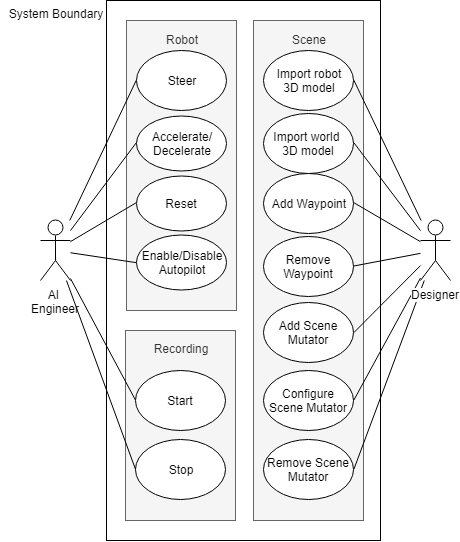
\includegraphics[width=10cm]{tex/img/ch04/Use_Cases_05.png}
\captionof{figure}{Use-Cases}
\label{fig:use-cases}
\end{center}

%////////////////////////////////////////////////
\section{Components}
Figure \ref{fig:use-cases} shows the high-level use-cases described in both modes, implicating the need for three high-level features (\ref{fig:component-diagram}): one that will be used to control robots (\textit{RobotController}), one that manages taking screenshots (\textit{Recording}) and one that allows designers to set up scenes (\textit{SceneManagement}).

\begin{center}
\noindent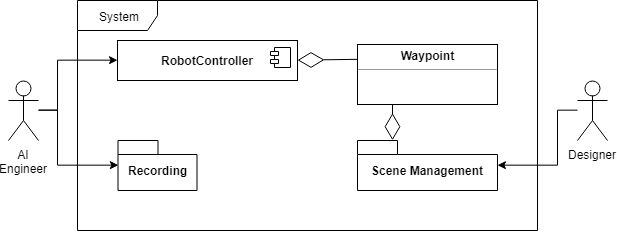
\includegraphics[width=12cm]{tex/img/ch04/Component_Diagram01.png}
\captionof{figure}{High-level component diagram}
\label{fig:component-diagram}
\end{center}

Refining the \textit{Recording}-package yields two components (\ref{fig:component-diagram-recording}): \textit{RenderingController} shall generate images from a robot's perspective and save them while \textit{ImageLabeller} adds \textit{Labels} to the images and saves them.

\begin{center}
\noindent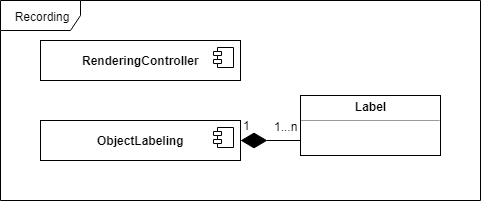
\includegraphics[width=12cm]{tex/img/ch04/Component_Diagram_Recording03.png}
\captionof{figure}{Recording-package}
\label{fig:component-diagram-recording}
\end{center}

The \textit{SceneManagement}-package also contains two components (\ref{fig:component-diagram-scenemanagement}): the \textit{MutationManager} manages the aforementioned mutators in scenes (e.g. triggering and resetting mutations), the \textit{WaypointManager} holds a list of paths consisting of multiple waypoints.

\begin{center}
\noindent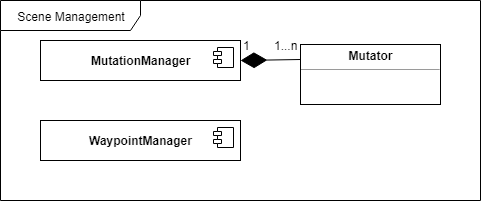
\includegraphics[width=12cm]{tex/img/ch04/Component_Diagram_SceneManagement02.png}
\captionof{figure}{SceneManagement-package}
\label{fig:component-diagram-scenemanagement}
\end{center}

%////////////////////////////////////////////////
%\section{Architecture}

%\subsection{Frontend: Game engine}

%\subsection{Backend: Renderer}